\documentclass[10pt,a4paper]{article}
\usepackage[margin=2.2cm]{geometry}
\usepackage[T1]{fontenc}
\usepackage{lmodern}
\usepackage{parskip}
\usepackage{booktabs}
\usepackage{tabularx}
\usepackage{array}
\usepackage{float}
\usepackage{graphicx}
\usepackage{enumitem}
\usepackage{xcolor}
\usepackage{xurl}
\usepackage[colorlinks=true,urlcolor=blue!60!black,linkcolor=black]{hyperref}

\graphicspath{{../figures/}}
\newcolumntype{R}{>{\raggedleft\arraybackslash}X}

\title{Drone Authentication Study --- Step 4 Progress Report\\[3pt]
\large Sequence diagrams of the drone authentication}
\author{}
\date{24 November 2026}

\begin{document}
\maketitle

\section*{Summary}

Steps 1--3 gave us numbers. Step 4 puts those numbers into pictures: three sequence diagrams that
show \emph{who sends what, in which order}, between the drone and the ground station. Every number
written on the diagrams was measured in Steps 1--3; nothing is guessed.

\begin{enumerate}[nosep]
  \item \textbf{Figure 1 --- the authentication protocol.} The five messages of one authentication
        (challenge, sign, send, verify, result), with the measured time and size of each part.
  \item \textbf{Figure 2 --- the same authentication as real packets.} Ed25519 against ML-DSA-44,
        drawn from the Wireshark recording of Step 3: 1 frame against 10 frames.
  \item \textbf{Figure 3 --- the whole drone mission.} Where authentication happens in a real
        flight, and where Step 5 (the MPU6050 sensor) fits in.
\end{enumerate}

% ---------------------------------------------------------------------------
\section{How to read a sequence diagram}

\begin{itemize}[nosep]
  \item Each box at the top is one device. The dashed line under it is that device over time.
  \item Time goes \textbf{downwards}.
  \item An arrow is a message from one device to the other. \textcolor[HTML]{2a78d6}{\textbf{Blue}}
        arrows come from the ground station, \textcolor[HTML]{eb6834}{\textbf{orange}} arrows come
        from the drone, grey dashed arrows happen only once before flight.
  \item A box on a line is work done inside one device (for example, signing).
\end{itemize}

% ---------------------------------------------------------------------------
\section{Figure 1: the authentication protocol}

\begin{figure}[H]
  \centering
  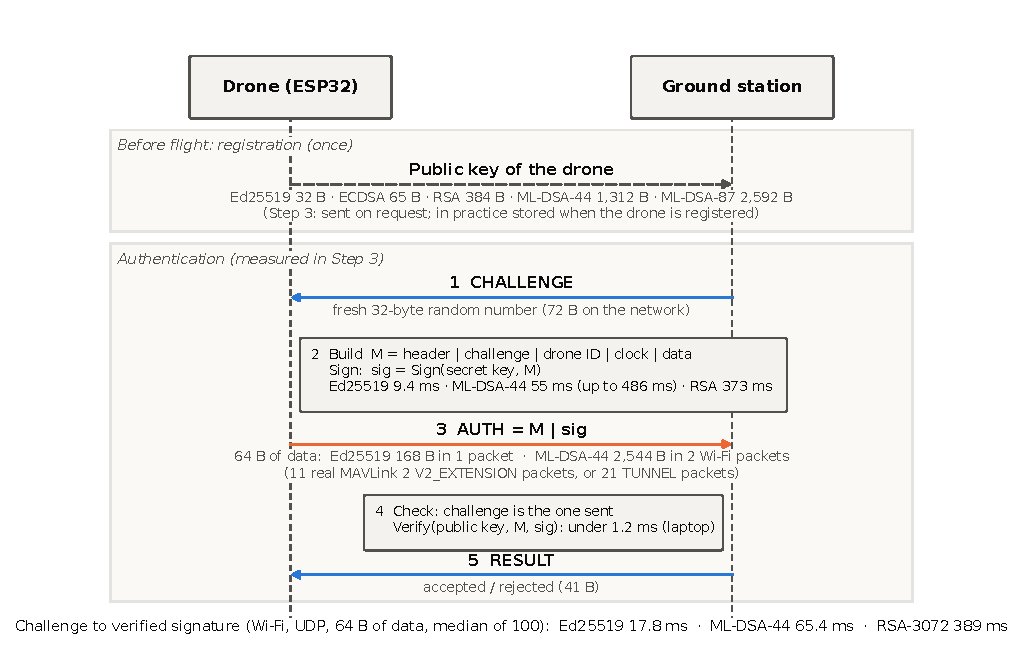
\includegraphics[width=0.92\linewidth]{fig8_seq_authentication.pdf}
  \caption{One drone authentication (challenge--response), exactly as tested in Step 3.}
\end{figure}

\textbf{What happens, step by step:}
\begin{enumerate}[nosep]
  \item \textbf{Registration (once, before flight).} The ground station stores the drone's public
        key. This key is small for the classical algorithms (32--384 bytes) and large for ML-DSA
        (1,312--2,592 bytes). Because it is sent only once, its size matters less.
  \item \textbf{Challenge.} The ground station sends a fresh 32-byte random number. A new number every
        time means an attacker cannot record an old answer and play it again (a \emph{replay attack}).
  \item \textbf{Sign.} The drone puts the challenge, its ID, its clock and the data together and
        signs them with its secret key. This is the slow part on the ESP32: 9.4\,ms for Ed25519,
        55\,ms for ML-DSA-44 (sometimes up to 486\,ms), 373\,ms for RSA-3072.
  \item \textbf{Send.} The signed message goes to the ground station. With 64 bytes of data it is
        168 bytes for Ed25519 but 2,544 bytes for ML-DSA-44 (2 Wi-Fi packets, or 10 MAVLink-sized
        frames).
  \item \textbf{Verify and answer.} The ground station checks that the challenge is the one it sent and
        that the signature is valid (under 1.2\,ms on the laptop), then answers accepted or rejected.
\end{enumerate}

\textbf{Total time} from challenge to verified signature on Wi-Fi (64 bytes of data, median):
Ed25519 19.5\,ms, ML-DSA-44 90.7\,ms, RSA-3072 440\,ms.

% ---------------------------------------------------------------------------
\section{Figure 2: the same authentication as real packets}

\begin{figure}[H]
  \centering
  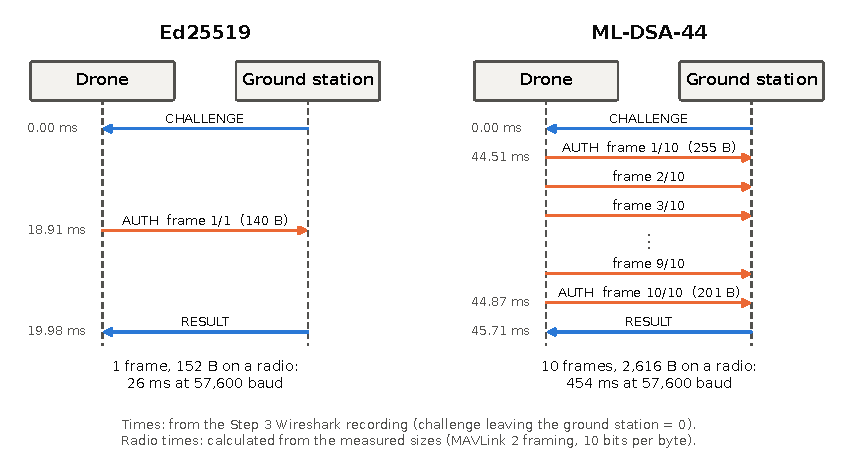
\includegraphics[width=\linewidth]{fig9_seq_packets.pdf}
  \caption{One real authentication with MAVLink-sized frames (at most 255 bytes each), 64 bytes of
  data. Times are from the Step 3 Wireshark recording. The drawing is not to scale in time.}
\end{figure}

\textbf{What it shows:}
\begin{itemize}[nosep]
  \item \textbf{Ed25519:} the whole answer is \textbf{1 frame} of 140 bytes. The drone needs about
        19\,ms (mostly signing), and the result comes back 1\,ms later.
  \item \textbf{ML-DSA-44:} the answer has to be cut into \textbf{10 frames}. On Wi-Fi all 10 leave
        within 0.4\,ms, because Wi-Fi is fast.
  \item \textbf{On a real drone radio it is very different.} Typical drone telemetry radios run at
        57.6\,kbit/s. At that speed the Ed25519 answer takes about \textbf{21\,ms} to send, but the
        ML-DSA-44 answer takes about \textbf{363\,ms}, and every one of the 10 frames must arrive.
        This is calculated from the measured sizes; we did not use a real telemetry radio.
\end{itemize}

% ---------------------------------------------------------------------------
\section{Figure 3: authentication in a drone mission}

\begin{figure}[H]
  \centering
  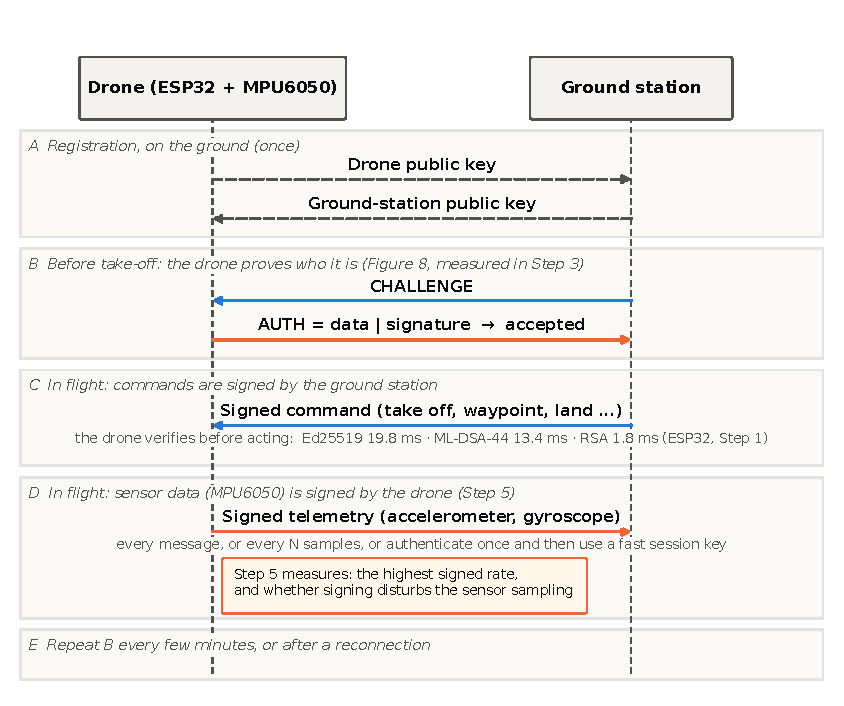
\includegraphics[width=0.8\linewidth]{fig10_seq_mission.pdf}
  \caption{Where signatures are used during a drone mission.}
\end{figure}

\textbf{The five parts:}
\begin{description}[nosep,leftmargin=1.2em,font=\normalfont\bfseries]
  \item[A --- Registration.] On the ground, the drone and the ground station exchange public keys once.
  \item[B --- Before take-off.] The drone proves who it is with the challenge--response of Figure 1.
        This is what we measured in Step 3.
  \item[C --- Commands in flight.] The ground station signs every command (take off, go to a waypoint,
        land). The drone checks the signature before it acts. On the ESP32 this check takes
        19.8\,ms for Ed25519, 13.4\,ms for ML-DSA-44 and 1.8\,ms for RSA-3072 (Step 1). Here ML-DSA-44
        is \emph{faster} than Ed25519.
  \item[D --- Sensor data in flight.] The drone signs its sensor readings (MPU6050 accelerometer and
        gyroscope). This is \textbf{Step 5}: we will measure how many signed messages per second the
        ESP32 can send, and whether signing disturbs the sensor sampling.
  \item[E --- Repeat.] Part B is repeated every few minutes, or after the link drops and comes back.
\end{description}

% ---------------------------------------------------------------------------
\section{What we learn from Step 4}

\begin{enumerate}[nosep]
  \item \textbf{The protocol is the same for every algorithm}; only the time and the size change.
        So the post-quantum algorithm can replace the classical one without changing the message
        flow.
  \item \textbf{The cost of ML-DSA is on the drone side and on the radio}: signing takes longer
        and the answer is 10--19 frames instead of 1. Checking is cheap on both sides.
  \item \textbf{Commands from the ground station are not a problem}: the drone verifies an ML-DSA-44
        command faster than an Ed25519 one.
  \item \textbf{The open question is signed sensor data}, sent many times per second. That is
        Step 5.
\end{enumerate}

\section*{Files}

{\small\ttfamily
Diagrams: results/e4/figures/ (fig8, fig9, fig10; PDF and PNG)\\
Script that draws them: tools/draw\_sequence\_diagrams.py
}

\end{document}
